%El objetivo de este documento es exponer el estudio de los puntos de funcion, para luego resumirlo en el plan de proyecto


\documentclass[spanish,a4paper,11pt, twoside]{report}	% Idioma, tamaño del papel, tamaño letra, documento (book, report, article, letter)

%%% PAQUETES
\usepackage[spanish,activeacute]{babel}				
% Babel: Adapta cosas como la tipografia, la fecha, lo de Chapter al español, y activeacute para apóstrofes (') como abreviaciones de acentos: \'{a}
\usepackage[utf8]{inputenc}					% Codificacion UTF8 (para meter tildes normal: á --> \'{a} )
\usepackage{multicol}						% Escritura en varias columnas
\usepackage{graphics}						% Inclusión de imágenes
\usepackage{graphicx}						% Mas para imagenes
\usepackage{geometry}						% Distribucion de la pagina: margenes, encabezados, tamaño pagina...
\usepackage{fancyhdr}						% Paquete para añadir y modificar encabezados y pies de pagina
\usepackage{hyperref}						% Para hipervínculos, en el indice al menos, GRACIAS A DAVID
%\usepackage{lastpage}						% Ultima pagina para poner, por ejemplo, 3 de 15
%%% PAQUETES MATEMATICOS
\usepackage{amsmath}						% Conjunto de paquetes desarrollados por la Amercian Matematical Society
\usepackage{amssymb}						% Tipografía mathbb y otros símbolos tambien de la AMS
\usepackage{amsthm}						% Paquete AMS theorem, de la AMS
\usepackage{amsfonts}						% Paquete con símbolos y mas, de la AMS
%\usepackage{nicefrac}						% Fracciones bonitas, LO DEJO COMENTADO PORQUE A VECES DA PROBLEMAS AL COMPILAR


%%% DECLARACIONES (sobre la forma de la pagina, encabezado etc.)
\pagenumbering{roman}						
% Para numerar las paginas en numeros romanos hasta que empiece el texto (tambien alph, Alph, roman, Roman...)
\pagestyle{fancy}							% Utiliza el paquete fancyhdr para encabezados y pies de pagina
%\thispagestyle{empty}  						% Para poner UNA pagina sin encabezados ni numero, "plain" CON numero, "fancy" normal
%\lhead{\section}							% Encabezado a la izquierda
%\fancyhead[RO,LE]{\bfseries Encabezado} 		%Encabezado de las páginas impares a la derecha y de las pares a la izquierda
\fancyhead[LO,RE]{\bfseries Documento UML} 	%Encabezado de las páginas impares a la izquierda y de las pares a la derecha
%\rhead{\bfseries ...}						%Encabezado a la derecha
\cfoot{\thepage}							% Numero de pagina centrado en el pie
%\cfoot{\thepage\ de \pageref{LastPage}}		% Numero de pagina centrado en el pie asi: n de m
\renewcommand{\headrulewidth}{0.4pt}			% Linea debajo del encabezado
\renewcommand{\footrulewidth}{0.4pt}			% Linea encima del pie de pagina
\renewcommand*{\thesection}{\arabic{section}}	% Hace que no apareca el indice de capitulos y que comience en section, GRACIAS A RUBEN
\newcommand*{\PKT}{\hbox{P}\kern-2.5pt\lower3.5pt\hbox{\small{K}}\kern-2.8pt\hbox{T}\kern-2pt}	%PiKey Team en bonito


%%%%% CUERPO %%%%%
\begin{document}

\title{\textbf{\huge{ Documento UML}} \\ 
	\textit{v3.0.1} \\	\vspace{0.1cm}
	\Large{Ingeniería del Software} \\
	
\includegraphics[scale=0.3]{ucm.pdf}}
\author{ {\Large{PiKey Team-}} \PKT \ : \vspace{0.2cm} \\
	Jesús Aguirre Pemán \\
	 Enrique Ballesteros Horcajo \\
	 Jaime Dan Porras Rhee \\
	 Ignacio Iker Prado Rujas \\
	 Alejandro Villarín Prieto }
\date{\Today}
\maketitle

\newpage
\mbox{}
\thispagestyle{empty}						% Hoja en blanco, sin numeros ni nada
\newpage


\tableofcontents 							%INDICE hipervinvulado

\pagenumbering{arabic}						% Pone el contador de paginas a 1 y ahora en numeros normales

%\vspace{0.35cm}
%\hspace{-3.2cm}
%\scalebox{0.85}{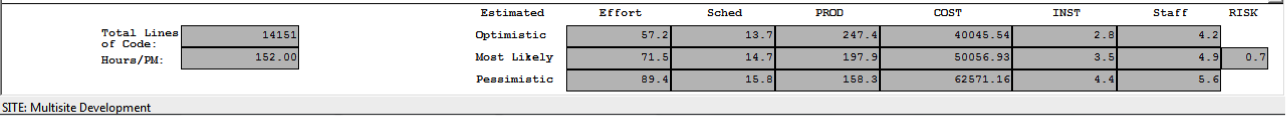
\includegraphics{COCOMOTODO1}} 
%\vspace{0.35cm}

\setcounter{section}{0}
\part{Introdución}
	\section{Propósito}
	Este documento pretende recopilar de manera clara y concisa todos los diagramas UML del Software KIKE HOSTELERIA ®, generados con la herramienta \texttt{Bouml}. Se pueden dividir en tres partes, cada una de ellas más cercana al código del lenguage de programación, y con mayor grado de detalle. Éstas son: Requisitos, análisis y diseño, partes fundamentales de este documento.

	\section{Audiencia} 
	La aplicación está pensada para hoteles y/o restaurantes de capacidad media/baja, pero podría ampliarse para capacidades mayores sin dificultad.

	El documento está pensado para dos audiencias distintas. En las primeras partes, sirve como lazo de comunicación entre el equipo (nosotros) y la empresa hostelera. Según se entra más en materia, centrándose en el Software, está pensado para el equipo de diseñadores y programadores.

	\section{Alcance}
	Todos los diagramas que se han requerido para la posterior codificación de la aplicación. Se añade, además, una breve explicación de los mismos, poniéndolos en contexto e indicando su naturaleza y significado.

	Todo el documento debe entenderse dentro del ámbito del UML y del modelo del Proceso Unificado, seguido durante todo el proyecto.

\section{Definiciones, acrónimos y abreviaturas}

	Todo lo referente a esta sección se encuentra en el documento anexo \texttt{Definiciones, acrónimos y abreviaturas}. Ahí se detallan las palabras poco comunes, los anglicísmos y abreviaturas que se emplean.

	\section{Referencias}
	Se han utilizado los diguientes recursos:
	\begin{itemize}
		\item Nuestro propio documento de \texttt{Documento de casos de uso}, así como \\ \texttt{Definiciones, acrónimos y abreviaturas}
		\item Apuntes de Clase de la asignatura “Ingeniería del Software" de la Universidad Complutense de Madrid, Curso 2012-2013
		\item \textbf{Booch, G.; Rumbaugh, J.; Jacobson, I. }. El lenguaje unificado de modelado (2006, 2ª edición).
		\item \textbf{Larman, C.}. UML y patrones (2003, 2ª edición).
		\item \textbf{Ambler, S. W.} The Elements of UML Style (2003).
	\end{itemize}

\newpage
\mbox{}
\thispagestyle{empty}						% Hoja en blanco, sin numeros ni nada
\newpage





\setcounter{section}{0}
\part{Requisitos}
	\begin{figure}[!h]
	\centering
	\includegraphics[scale=0.5]{modelodedominio.png}
	\vspace{-1.25 true cm}
	\caption{Modelo de dominio}
	\end{figure}	\section{Modelo de Dominio}
	En esta sección se recoge el modelo de dominio de toda la aplicación. De izquierda a derecha, podemos ver la relación entre el cliente y las reservas que puede hacer, tanto del restaurante como del hotel. A partir de ellas se puede genarar una factura. 

	Las reservas del hotel son atendidas por el recepcionista, y las del restaurante por el camarero (o en su defecto, el maître). El camarero, además tiene varias posibilidades, puede acceder y modificar la distribución de las mesas del restaurante, tomar o modificar comandas, ver o modificar el menú y ver o modificar las existencias de la cocina y el bar.

	En cuanto a la limpieza, el encargado asigna tareas de limpieza al personal de limpieza. Posteriormente, cuando se suponen completadas, el encargado revisa si se han cumplido los objetivos en dichos encargos, dando su visto bueno.

	Además, el encargado de mantenimiento puede ver las tareas que tiene pendientes por resolver en el hotel o el restaurante. Estas son notificadas por el resto de empleados (o el mismo, al ser un empleado más) cuando las descubren. Otro medio de comunicación entre los empleados son las notas. Cualquiera puede escribir una y cualquiera puede verlas. Su fin es distinto al de las obligaciones de mantenimiento, ya que pueden tratarse temas más triviales o que no tocan dichas tareas.
		
	Por último, el jefe del negocio tiene acceso a las cuentas de las cajas de la recepción y del restaurante, que se recogen en el libro diario de la aplicación. Éste, a su vez, se resume en el libro mayor.




	\section{Diagramas de actividad}
	No consideramos necesarios estos diagramas, ya que creemos que la información que aportan ya la dan los diagramas de secuencia junto con la documentación.



\setcounter{section}{0}
\part{Análisis}
	\section{Diagamas de paquetes}
	En la aplicación hay una clara brecha entre la lógica y la interfaz de la misma, más nítida por el uso del patrón Modelo-Vista-Controlador (ver Parte V para más información). Esto se refleja en el diagrama de paquetes. Además, en la lógica se distinguen a su vez dos partes, lo relativo a los empleados y lo relativo a las cuentas del negocio. Cada una de estas partes incluye lo que indica el diagrama.
	\begin{figure}[!h]
	\centering
	\includegraphics[scale=0.15]{diagramadepaquetes.png}	
	\caption{Diagrama de paquetes}
	\end{figure}

	\section{Diagramas de comunicación}
		\subsection{Menú del restaurante}

		\begin{figure}[!h]
		\centering
		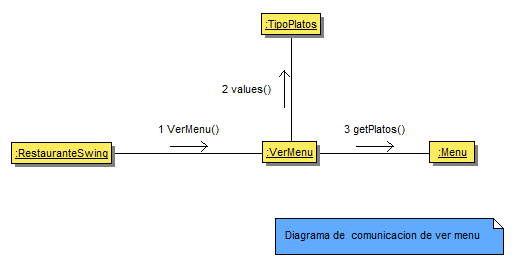
\includegraphics[scale=0.5]{DCvermenu.png}
		\caption{Diagrama de comunicación del menú}
		\end{figure}
		Desde el menú principal se accede a la vista del menú que le solicita los datos a la clase Menú.
		Requiere los tipos de plato existentes y las consumiciones de cada tipo de plato. 

		\begin{figure}[!h]
		\centering
		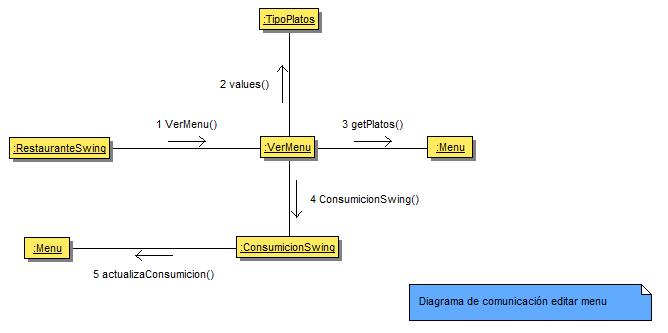
\includegraphics[scale=0.5]{DCeditarmenu.png}
		\caption{Diagrama de comunicación de modificar el menú}
		\end{figure}
		Se accede  a la pestaña de ver menú que reúne los datos del Menú y te
		permite editar los campos de las consumiciones que se quiera a través de una
		interfaz.

		\begin{figure}[!h]
		\centering
		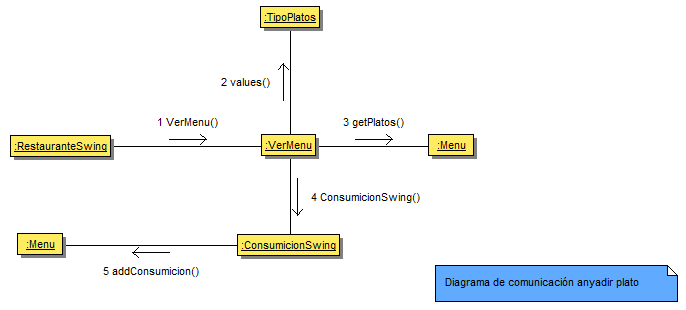
\includegraphics[scale=0.5]{DCanyadirconsumicion.png}
		\caption{Diagrama de comunicación de añadir plato al menú}
		\end{figure}
		Accediendo a la pestaña ver menú, que reúne los datos de la clase Menú, te
		permite añadir consumiciones a ésta a través de una interfaz.

		\begin{figure}[!h]
		\centering
		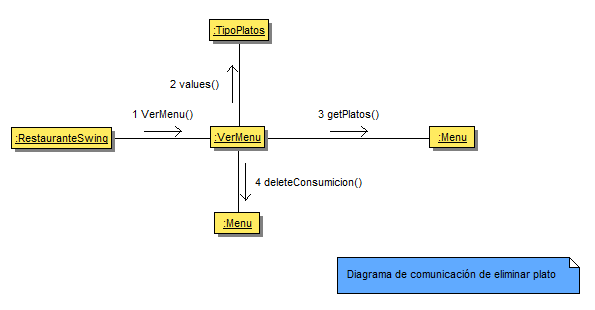
\includegraphics[scale=0.5]{DCeliminarconsumicion.png}
		\caption{Diagrama de comunicación de eliminar consumición}
		\end{figure}
		A través de la interfaz de ver menú que reúne las consumiciones del menú, te permite
		eliminar cualquier plato de este.

		\subsection{Reservas del restaurante}

		\begin{figure}[!h]
		\centering
		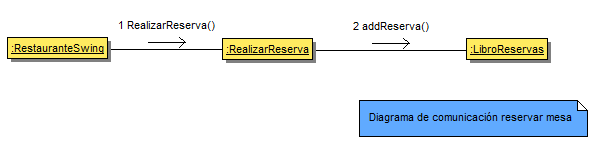
\includegraphics[scale=0.5]{DCreserva.png}
		\caption{Diagrama de comunicación de reservar una mesa}
		\end{figure}
		A través de la interfaz realizar reserva, que te permite rellenar los campos de 
		una, se añade al libro de reservas que acumula todas.

		\begin{figure}[!h]
		\centering
		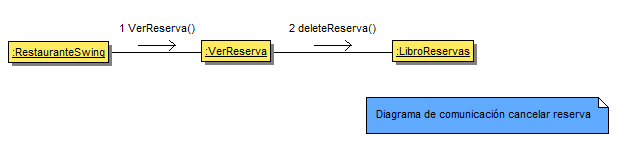
\includegraphics[scale=0.5]{DCeliminarreserva.png}
 		\caption{Diagrama de comunicación de anular reserva del restaurante}
		\end{figure}
		Accediendo desde la ventana principal, ver reserva te ofrece la posibilidad de eliminar la reserva deseada del libro de reservas.

		\subsection{Comandas del restaurante}

		\begin{figure}[!h]
		\centering
		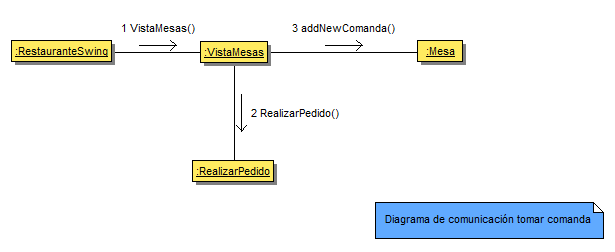
\includegraphics[scale=0.5]{DCcomanda.png}
		\caption{Diagrama de comunicación de tomar comanda}
		\end{figure}
		Desde la ventana principal se accede a la vista de las mesas, que tras haber seleccionado una contacta con realizar
		pedido que te permite crear una comanda. Una vez creada, la vista de las mesas se la envía a la mesa para que la almacene.

		\begin{figure}[!h]
		\centering
		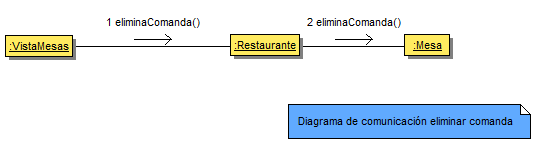
\includegraphics[scale=0.5]{DCeliminarcomanda.png}
		\caption{Diagrama de comunicación de eliminar comanda}
		\end{figure}
		Desde la vista de las mesas se selecciona una comanda y se notifica a la mesa su borrado.

		\subsection{Factura del restaurante}

		\begin{figure}[!h]
		\centering
		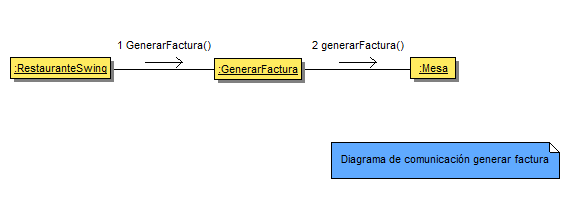
\includegraphics[scale=0.5]{DCfactura.png}
		\caption{Diagrama de comunicación de generar factura del restaurante }
		\end{figure}
		Desde la ventana principal se accede a generar factura, donde se selecciona la mesa de la cual se quiere cobrar 
		la factura, a quien se le solicita ésta para gestionarla desde generar factura.

		\subsection{Incidencias de mantenimiento}

		\begin{figure}[!h]
		\centering
		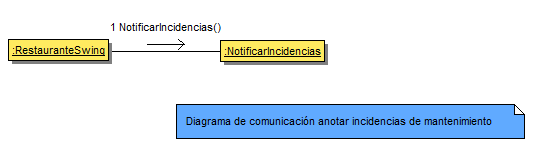
\includegraphics[scale=0.5]{DCanotarincidencias.png}
		\caption{Diagrama de comunicación de mantenimiento}
		\end{figure}
		Se  crea una nota de texto al acceder a notificar incidencias que te permite indicar tu problema.





	\section{Diagramas de clases de análisis}
		\subsection{Menú del restaurante}
		El camarero puede ver los elementos del menú, así como modificarlos (que implica verlos). Para ello se accede al menú, que lleva los distintos tipos de consumiciones, que son bebidas, primeros, segundos y postres.
		\begin{figure}[!h]
		\centering
		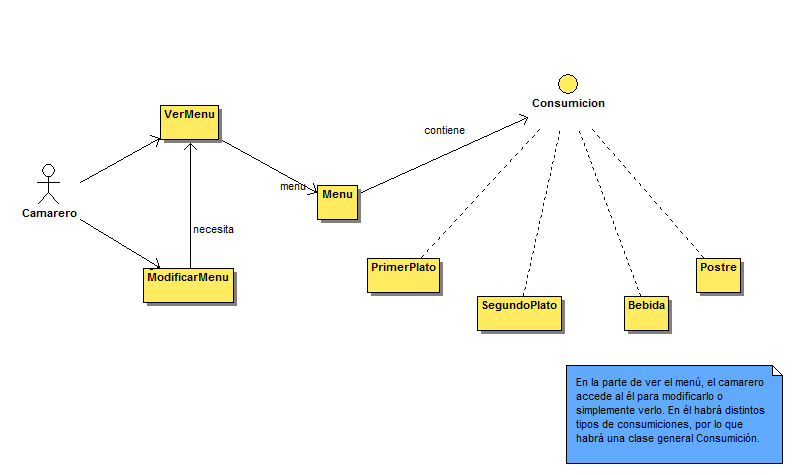
\includegraphics[scale=0.5]{DCAmenu.png}
		\caption{Diagrama de clases de análisis del menú}
		\end{figure}

		\subsection{Reservas del restaurante}
		El maître, o el camarero, puede añadir, modificar o eliminar reservas al libro de reservas, que es el sitio donde están todas las reservas. Cada reserva lleva asociada una fecha.
		\begin{figure}[!h]
		\centering
		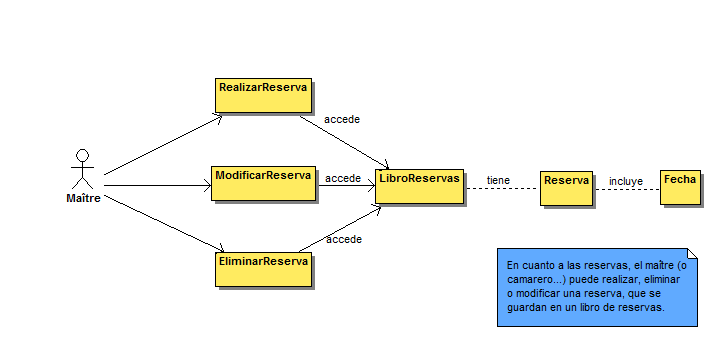
\includegraphics[scale=0.5]{DCAresevas.png}
		\caption{Diagrama de clases de análisis de las reservas del restaurante}
		\end{figure}

		\subsection{Comandas del restaurante}
		El camarero puede realizar o modificar una comanda. Ese pedido se le asocia a una mesa determinada. La comanda en cuestion lleva un conjunto de consumiciones que se extraen del menú.
		\begin{figure}[!h]
		\centering
		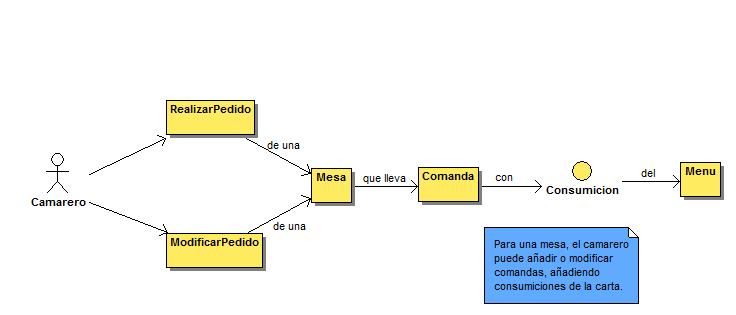
\includegraphics[scale=0.5]{DCAcomandas.png}
		\caption{Diagrama de clases de análisis de las comandas}
		\end{figure}

		\subsection{Factura del restaurante}
		Esta operación es sencilla. Llegado el momento de pagar, se pide que se genere una factura de una determinada mesa. Entonces se recopilan las consumiciones de esa mesa y se extrae el total a pagar.
		\begin{figure}[!h]
		\centering
		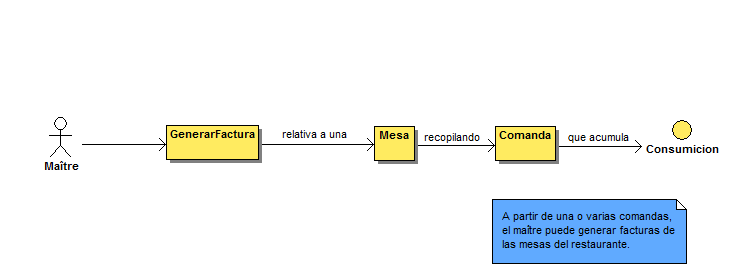
\includegraphics[scale=0.5]{DCAfactura.png}
		\caption{Diagrama de clases de análisis de las facturas}
		\end{figure}




\setcounter{section}{0}
\part{Diseño}
	\section{Diagramas de secuencia}
		\subsection{Menú del restaurante}
		La acción se inicia en la interfaz RestauranteSwing, que le pide al menú que desea verlo. Este le devolverá una lista con la información de qué tipos de consumiciones hay, para mostrarlos. Posteriormente, se notificará qué tipo de consumición se desea ver. En el bucle se le pide uno a uno los nombres de cada consumición de ese tipo, y opcionalmente se pedirá que muestre la descripción de alguno. 
		\begin{figure}[!h]
		\centering
		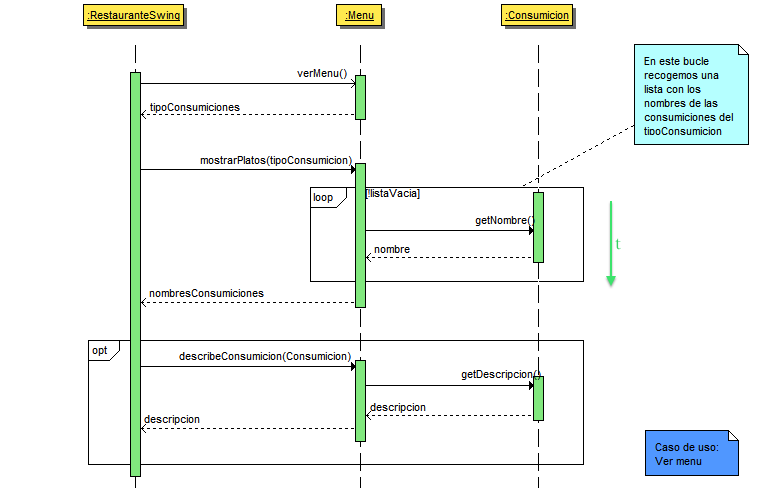
\includegraphics[scale=0.5]{DSvermenu.png}
		\caption{Diagrama de secuencia del menú}
		\end{figure}

		También se permite, como se ha dicho numerosas veces, modificar el menú. Hay tres opciones distintas para ello, a saber, añadir una nueva consumición, eliminar una existente o modificarla. Por claridad, cada una de estos opciones está en un diagrama distinto. El camino siempre es el mismo: de la interfaz al controlador, y de éste al menú. Cabe destacar que al modificar una consumición puedes cambiar el nombre, la descripción o el precio.
		\begin{figure}[!h]
		\centering
		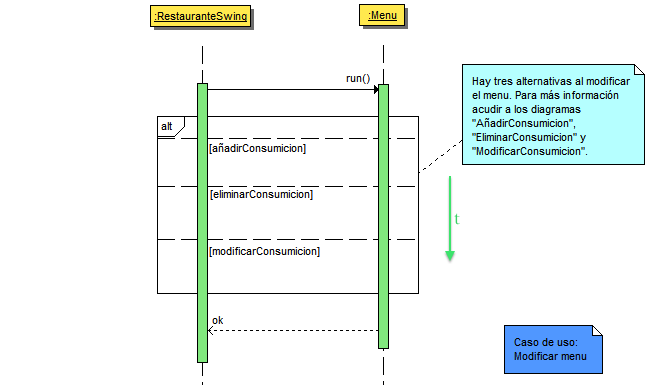
\includegraphics[scale=0.5]{DSmodificarmenu.png}
		\caption{Diagrama de secuencia de modificar menú}
		\end{figure}		

		\begin{figure}[!h]
		\centering
		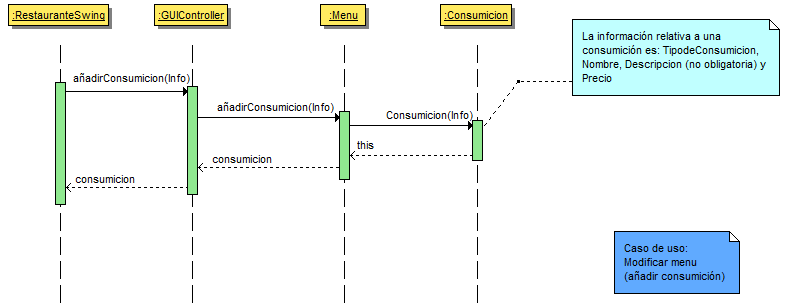
\includegraphics[scale=0.5]{DSanyadirconsumicion.png}
		\caption{Diagrama de secuencia de modificar menú (añadir consumición)}
		\end{figure}

		\begin{figure}[!h]
		\centering
		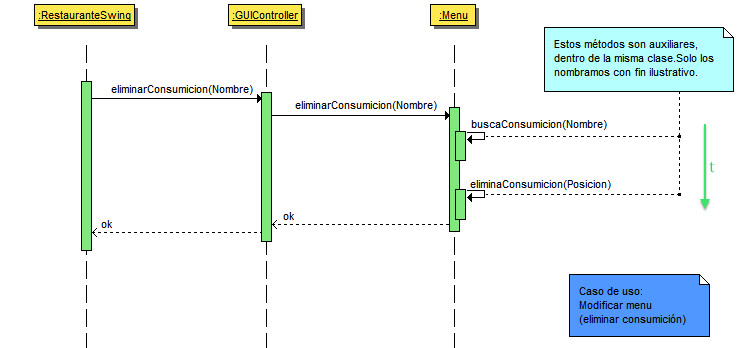
\includegraphics[scale=0.5]{DSeliminarconsumicion.png}
		\caption{Diagrama de secuencia de modificar menú (eliminar consumición)}
		\end{figure}

		\begin{figure}[!h]
		\centering
		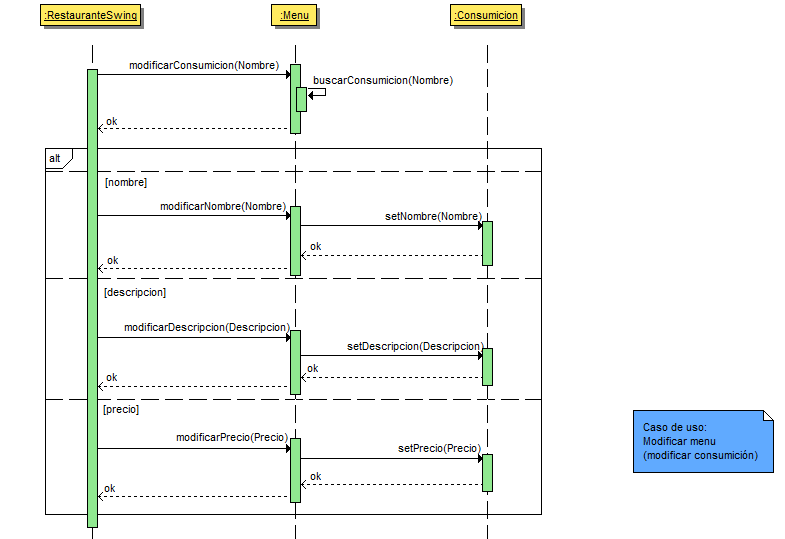
\includegraphics[scale=0.5]{DSmodificarconsumicion.png}
		\caption{Diagrama de secuencia de modificar menú (modificar consumición)}
		\end{figure}


		\subsection{Reservas del restaurante}
		Para ver las reservas,  como siempre hacemos debido al M-V-C, la interfaz RestauranteSwing se lo pide al controlador, y este se lo pide al Restaurante, que lleva una lista con las reservas.
		\begin{figure}[!h]
		\centering
		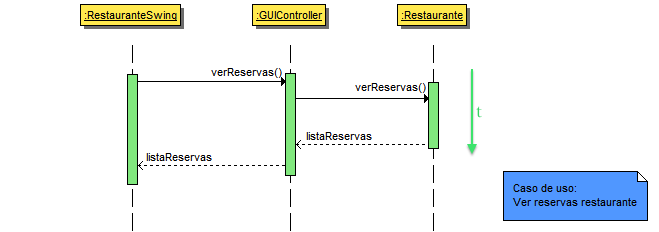
\includegraphics[scale=0.5]{DSverreservas.png}
		\caption{Diagrama de secuencia de ver las reservas del restaurante}
		\end{figure}

		Para hacer una reserva, el proceso es el mismo, sólo que se llama además al constructor de la reserva. Una vez creada se añade si es posible (puede que para la fecha solicitada se haya llenado ya el cupo de reservas). La anulación de una reserva es análoga.
		\begin{figure}[!h]
		\centering
		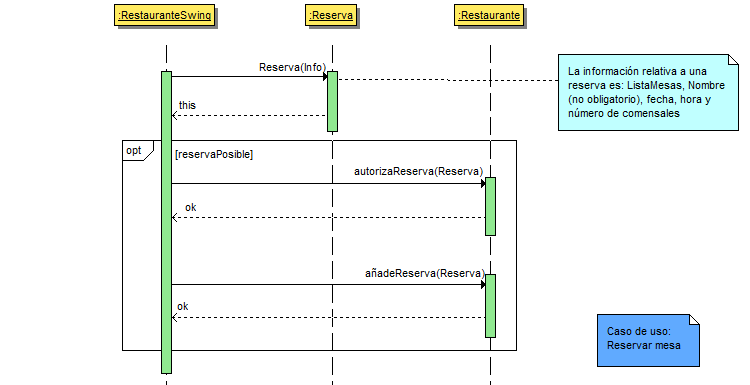
\includegraphics[scale=0.5]{DSreservarmesa.png}
		\caption{Diagrama de secuencia de reservar mesa del restaurante}
		\end{figure}

		\begin{figure}[!h]
		\centering
		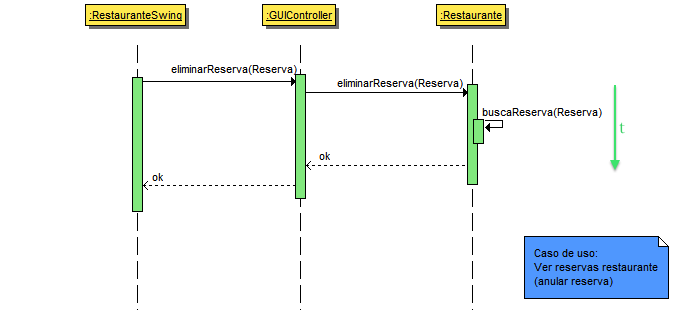
\includegraphics[scale=0.5]{DSanularreserva.png}
		\caption{Diagrama de secuencia de anular reservas del restaurante}
		\end{figure}

		


		\subsection{Comandas del restaurante}
		Para tomar una comanda, RestauranteSwing se lo solicita al GUIController, pasándole las consumiciones y la mesa a la que le corresponden. Este se lo pasa al restaurante, que llama al constructor de comanda con la lista de consumiciones. Finalmente se añade la comanda a la mesa antes mencionada.
		\begin{figure}[!h]
		\centering
		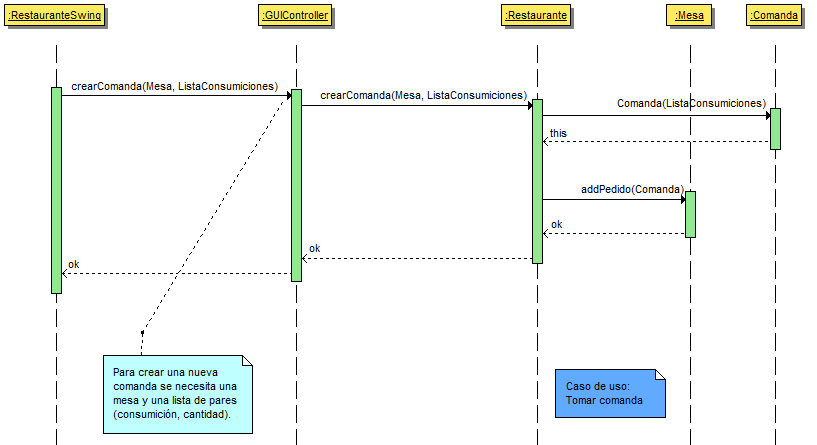
\includegraphics[scale=0.5]{DStomarcomanda.png}
		\caption{Diagrama de secuencia de tomar comanda }
		\end{figure}

		El proceso es el mismo, pero en vez de llamar al constructor de la comanda, se elimina de la mesa correspondiente.
		\begin{figure}[!h]
		\centering
		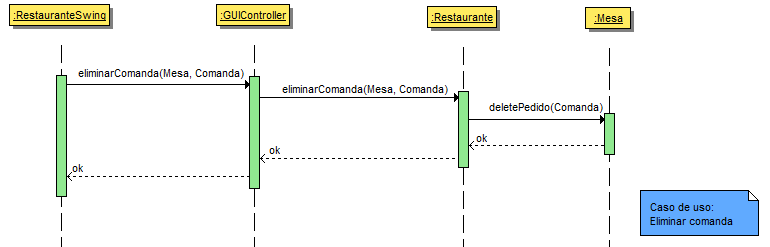
\includegraphics[scale=0.5]{DSeliminarcomanda.png}
		\caption{Diagrama de secuencia de eliminar comanda}
		\end{figure}

		Esta parte está en fase de pruebas, pero ya tiene su diagrama de secuencia definido. Permite añadir o eliminar consumiciones de la comanda correspondiente a una mesa. Nótese que es indiferente si la consumición existía ya o se trata de algo que ya se había pedido (como por ejemplo una botella de agua) y se incrementa su cantidad.
		\begin{figure}[!h]
		\centering
		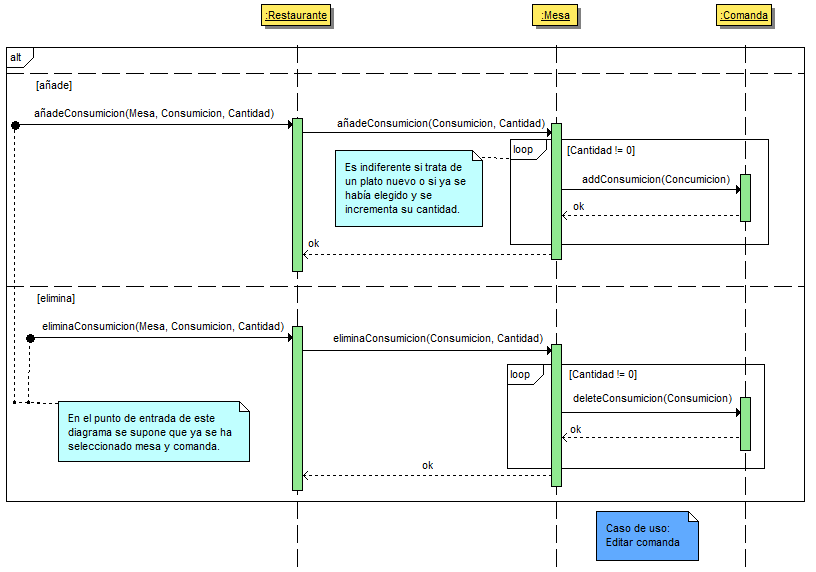
\includegraphics[scale=0.5]{DSmodificarcomanda.png}
		\caption{Diagrama de secuencia de modificar comanda}
		\end{figure}


		
		\subsection{Factura del restaurante}
		La clase RestauranteGUI llama al controlador, pasándole la mesa de la que se quiere extraer la factura. Éste transmite el mensaje al restaurante, donde se encuentra la mesa en cuestión. Sobre ella, se llama a la clase factura, que ordena la lista de comandas que recibe. Simplemente recorre tipos de platos (primero bebidas, luego primeros...) y para cada uno, recorre las comandas, recogiendo la consumición que toque. Devuelve la cadena con la factura total.
		\begin{figure}[!h]
		\centering
		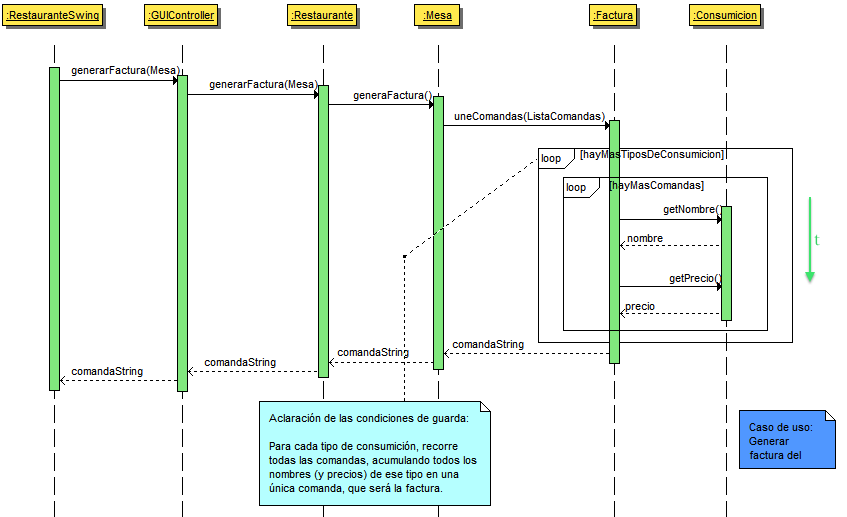
\includegraphics[scale=0.5]{DSfactura.png}
		\caption{Diagrama de secuencia de generar factura del restaurante}
		\end{figure}


		\subsection{Recuento de existencias}
		Esta parte no se implementa en esta versión, pero está en fase de desarrollo para presentársela al cliente como complemento. Simplemente habría una lista con las existencias, que tienen una cantidad asociada. En caso de necesitar modificar una de estas cantidades, la interfaz llama al controlador, que llama al inventario (donde esta las exitencias) y se cambia la cantidad de la que corresponda.
		\begin{figure}[!h]
		\centering
		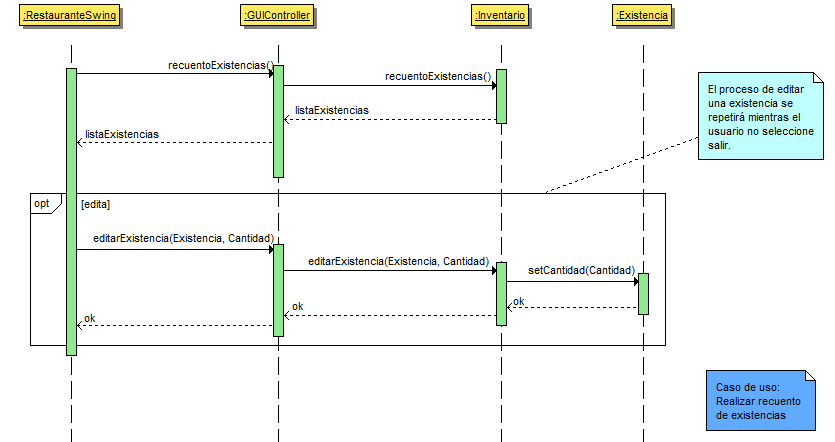
\includegraphics[scale=0.5]{DSexistencias.png}
		\caption{Diagrama de secuencia de realizar recuento de existencias del restaurante}
		\end{figure}



	\section{Diagramas de clases de diseño}
		\subsection{Menú del restaurante}
		\begin{figure}[!h]
		\centering
		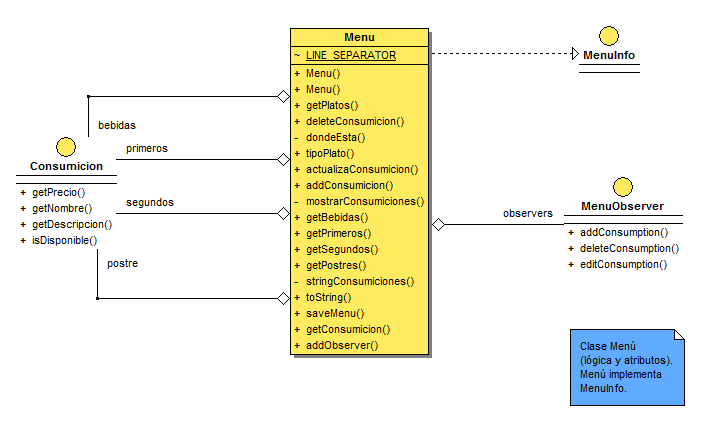
\includegraphics[scale=0.5]{DCDmenu.png}
		\caption{Diagrama de clases de diseño de la lógica del menú}
		\end{figure}

		\begin{figure}[!h]
		\centering
		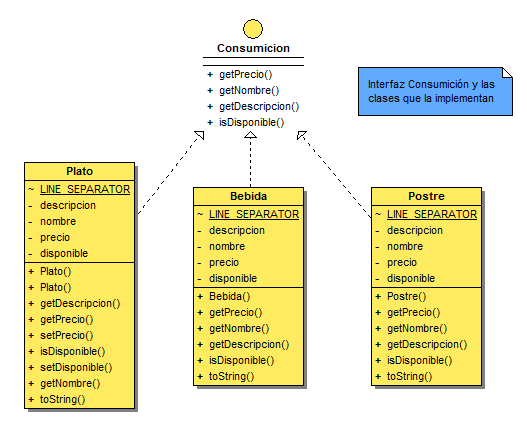
\includegraphics[scale=0.5]{DCDconsumicion.png}
		\caption{Diagrama de clases de diseño de las consumiciones}
		\end{figure}

		\begin{figure}[!h]
		\centering
		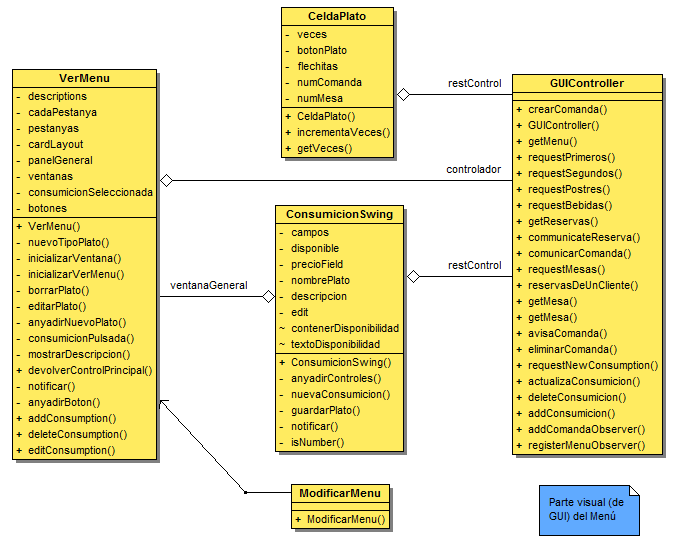
\includegraphics[scale=0.5]{DCDvistamenu.png}
		\caption{Diagrama de clases de diseño de la interfaz del menú }
		\end{figure}


		\subsection{Reservas del restaurante}
		\begin{figure}[!h]
		\centering
		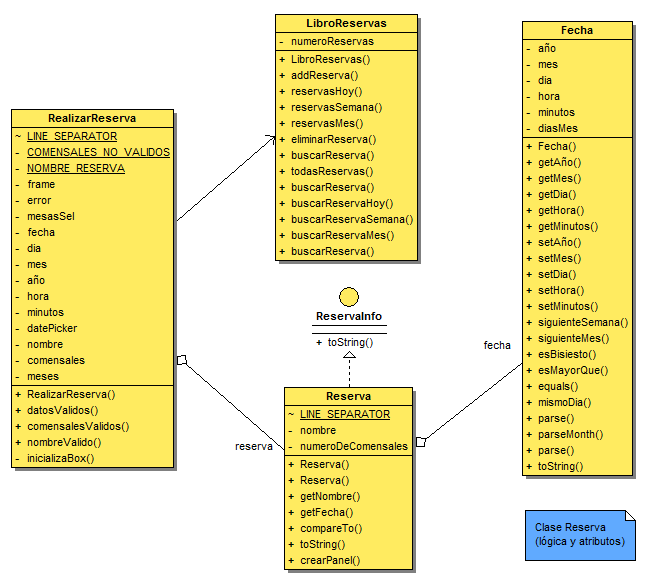
\includegraphics[scale=0.5]{DCDreservas.png}
		\caption{Diagrama de clases de diseño de la lógica de las reservas}
		\end{figure}

		\begin{figure}[!h]
		\centering
		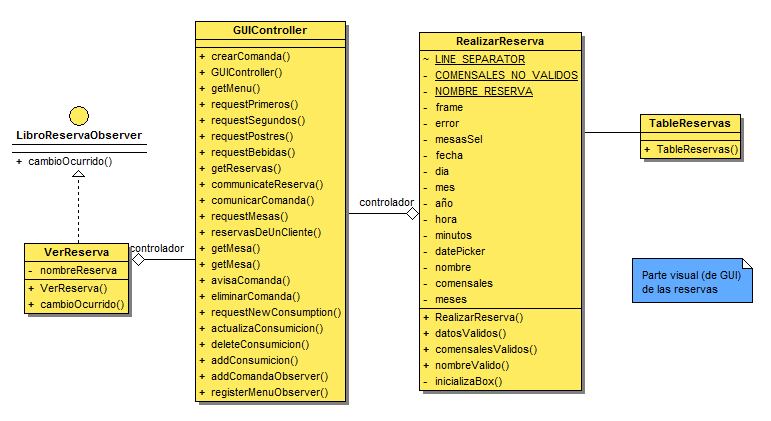
\includegraphics[scale=0.5]{DCDvistareservas.png}
		\caption{Diagrama de clases de diseño de la interfaz de las reservas}
		\end{figure}

		\subsection{Comandas del restaurante}
		\begin{figure}[!h]
		\centering
		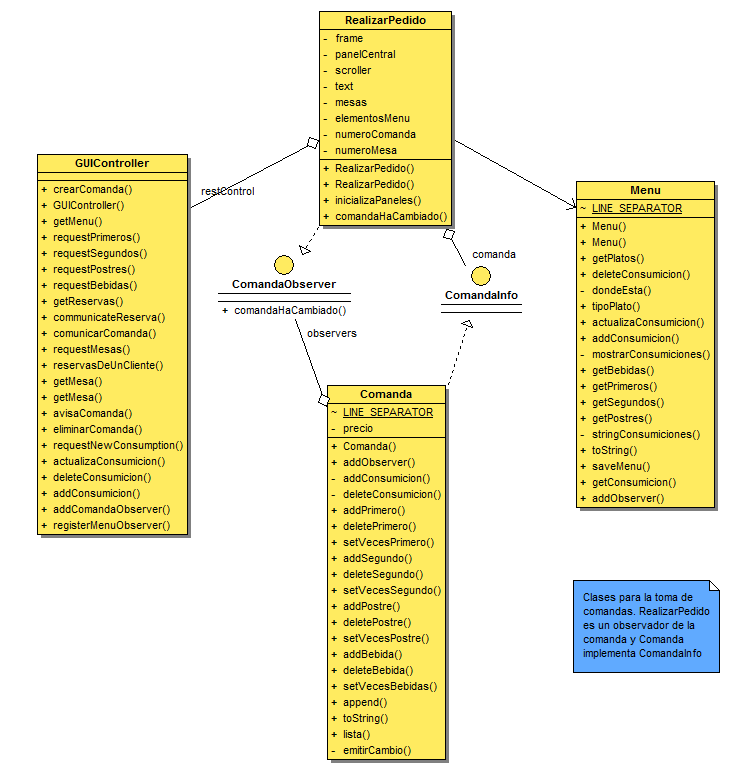
\includegraphics[scale=0.5]{DCDcomandas.png}
		\caption{Diagrama de clases de diseño de las comandas}
		\end{figure}

		\begin{figure}[!h]
		\centering
		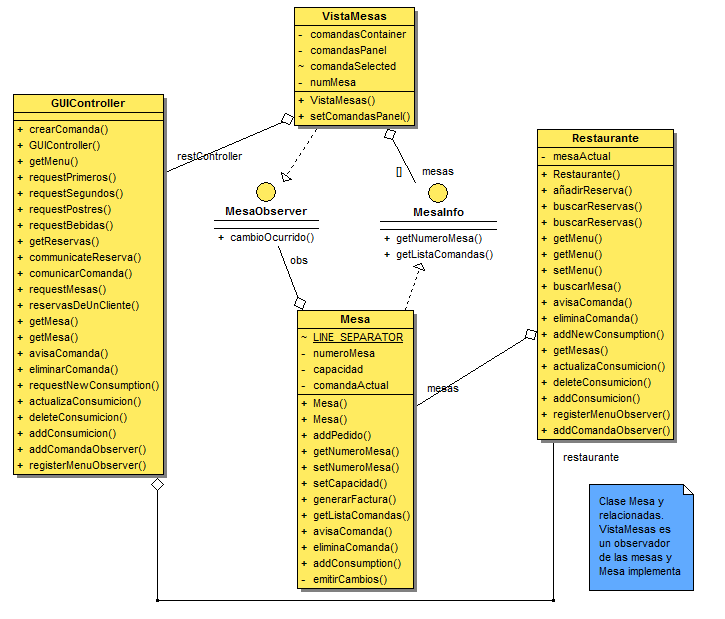
\includegraphics[scale=0.5]{DCDmesas.png}
		\caption{Diagrama de clases de diseño de las mesas}
		\end{figure}
\clearpage
		\subsection{Factura del restaurante}
		\begin{figure}[!h]
		\centering
		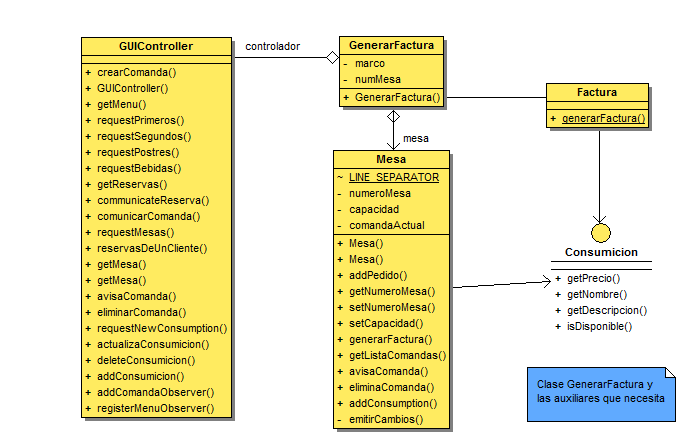
\includegraphics[scale=0.5]{DCDfactura.png}
		\caption{Diagrama de clases de diseño de generar facturas del restaurante}
		\end{figure}

		\subsection{Cargadores de ficheros}
		\begin{figure}[!h]
		\centering
		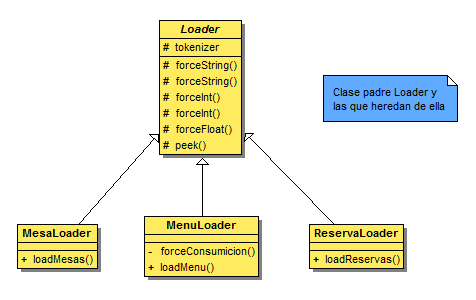
\includegraphics[scale=0.5]{DCDloader.png}
		\caption{Diagrama de clases de diseño de los cargadores de ficheros}
		\end{figure}

	\section{Diagramas de componentes}
	No se consideran necesarios.

	\section{Diagramas de despliegue}
	No se consideran necesarios puesto que la aplicación no tiene la complejidad necesaria.





\setcounter{section}{0}
\part{Patrones de diseño}



\newpage
\mbox{}
\thispagestyle{empty}						% Hoja en blanco, sin numeros ni nada al final del documento
\newpage

\end{document}